\section{Selection t-SNE Visualizations}
\label{app:selection-tsne}

Before measuring selected-set overlap directly, we first visualize the selected subsets in a shared low-dimensional embedding space. These plots are qualitative: the t-SNE coordinates~\citep{van2008visualizing} are computed from lightweight image proxy embeddings and are used only for visualization, not for the selection-overlap metric below. Gray points denote source candidates, and colored points denote the subset selected by each method.

The ratio-$0.10$ plots in Figures~\ref{fig:tsne-r01-coco} and~\ref{fig:tsne-r01-kitti} show the selected subsets for COCO and KITTI. The ratio-$0.05$ KITTI plots in Figures~\ref{fig:tsne-r005-kitti} and~\ref{fig:tsne-overlay-r005-kitti} provide a more stringent small-budget view, with the overlay figure making the separation between \model and representative active-learning baselines easier to inspect.

The visual pattern should be interpreted in light of the selection score in Section~\ref{subsec:slice-enrichment}. \model is not designed to be a uniformly spread coreset in the t-SNE plane. It behaves more like an attribute-conditioned real-source search: the selected images are related to the repair attributes, but they are spread across more diverse backgrounds, classes, and nearby contexts. The rarity term $\textcolor{colorR}{R_{i,a}}$ intentionally gives higher priority to source examples whose attribute values are rare within their class, so \model can place more mass on peripheral or less common regions of the proxy embedding. These peripheral selections are consistent with the intended rare-case behavior, although the t-SNE plot alone should be read only as a qualitative diagnostic. The penalty term $\textcolor{colorP}{P_{i,a}}$ reduces the priority of attribute values already supplied by the generated pool, so the selected source points are encouraged to complement the synthetic repair data instead of repeating it. Finally, the soft class-balance correction $\textcolor{colorC}{C_c^{(k)}}$ pulls the greedy selection away from a single high-scoring class or local region. Thus the expected signature is controlled non-uniformity: \model may put more mass on visually or semantically unusual regions than random, uncertainty, or pure coverage baselines, while still retaining cross-class coverage through the balance term.

The KITTI overlay illustrates this qualitative behavior. The \model points do not simply trace the same support as the representative active-learning baselines; they are shifted toward a different subset of the proxy embedding space, including some less central regions. This is consistent with the score's purpose: select real source images that are attribute-relevant and sufficiently diverse to support retraining, with extra weight on rare repair-relevant cases. Because t-SNE is only a two-dimensional proxy visualization, this observation is not a standalone performance claim. It motivates the direct selected-set overlap analysis in Section~\ref{app:overlap-diagnostic}, where the same conclusion is tested through Jaccard overlap between selected subsets.

These visualizations should not be interpreted as proof that low overlap improves downstream repair. They instead provide a sanity check that \model is not visibly collapsing onto the same region as the standard active-learning selectors. The quantitative version of this diagnostic is the Jaccard analysis in Section~\ref{app:overlap-diagnostic}.

% \begin{figure}[p]
% \centering
% 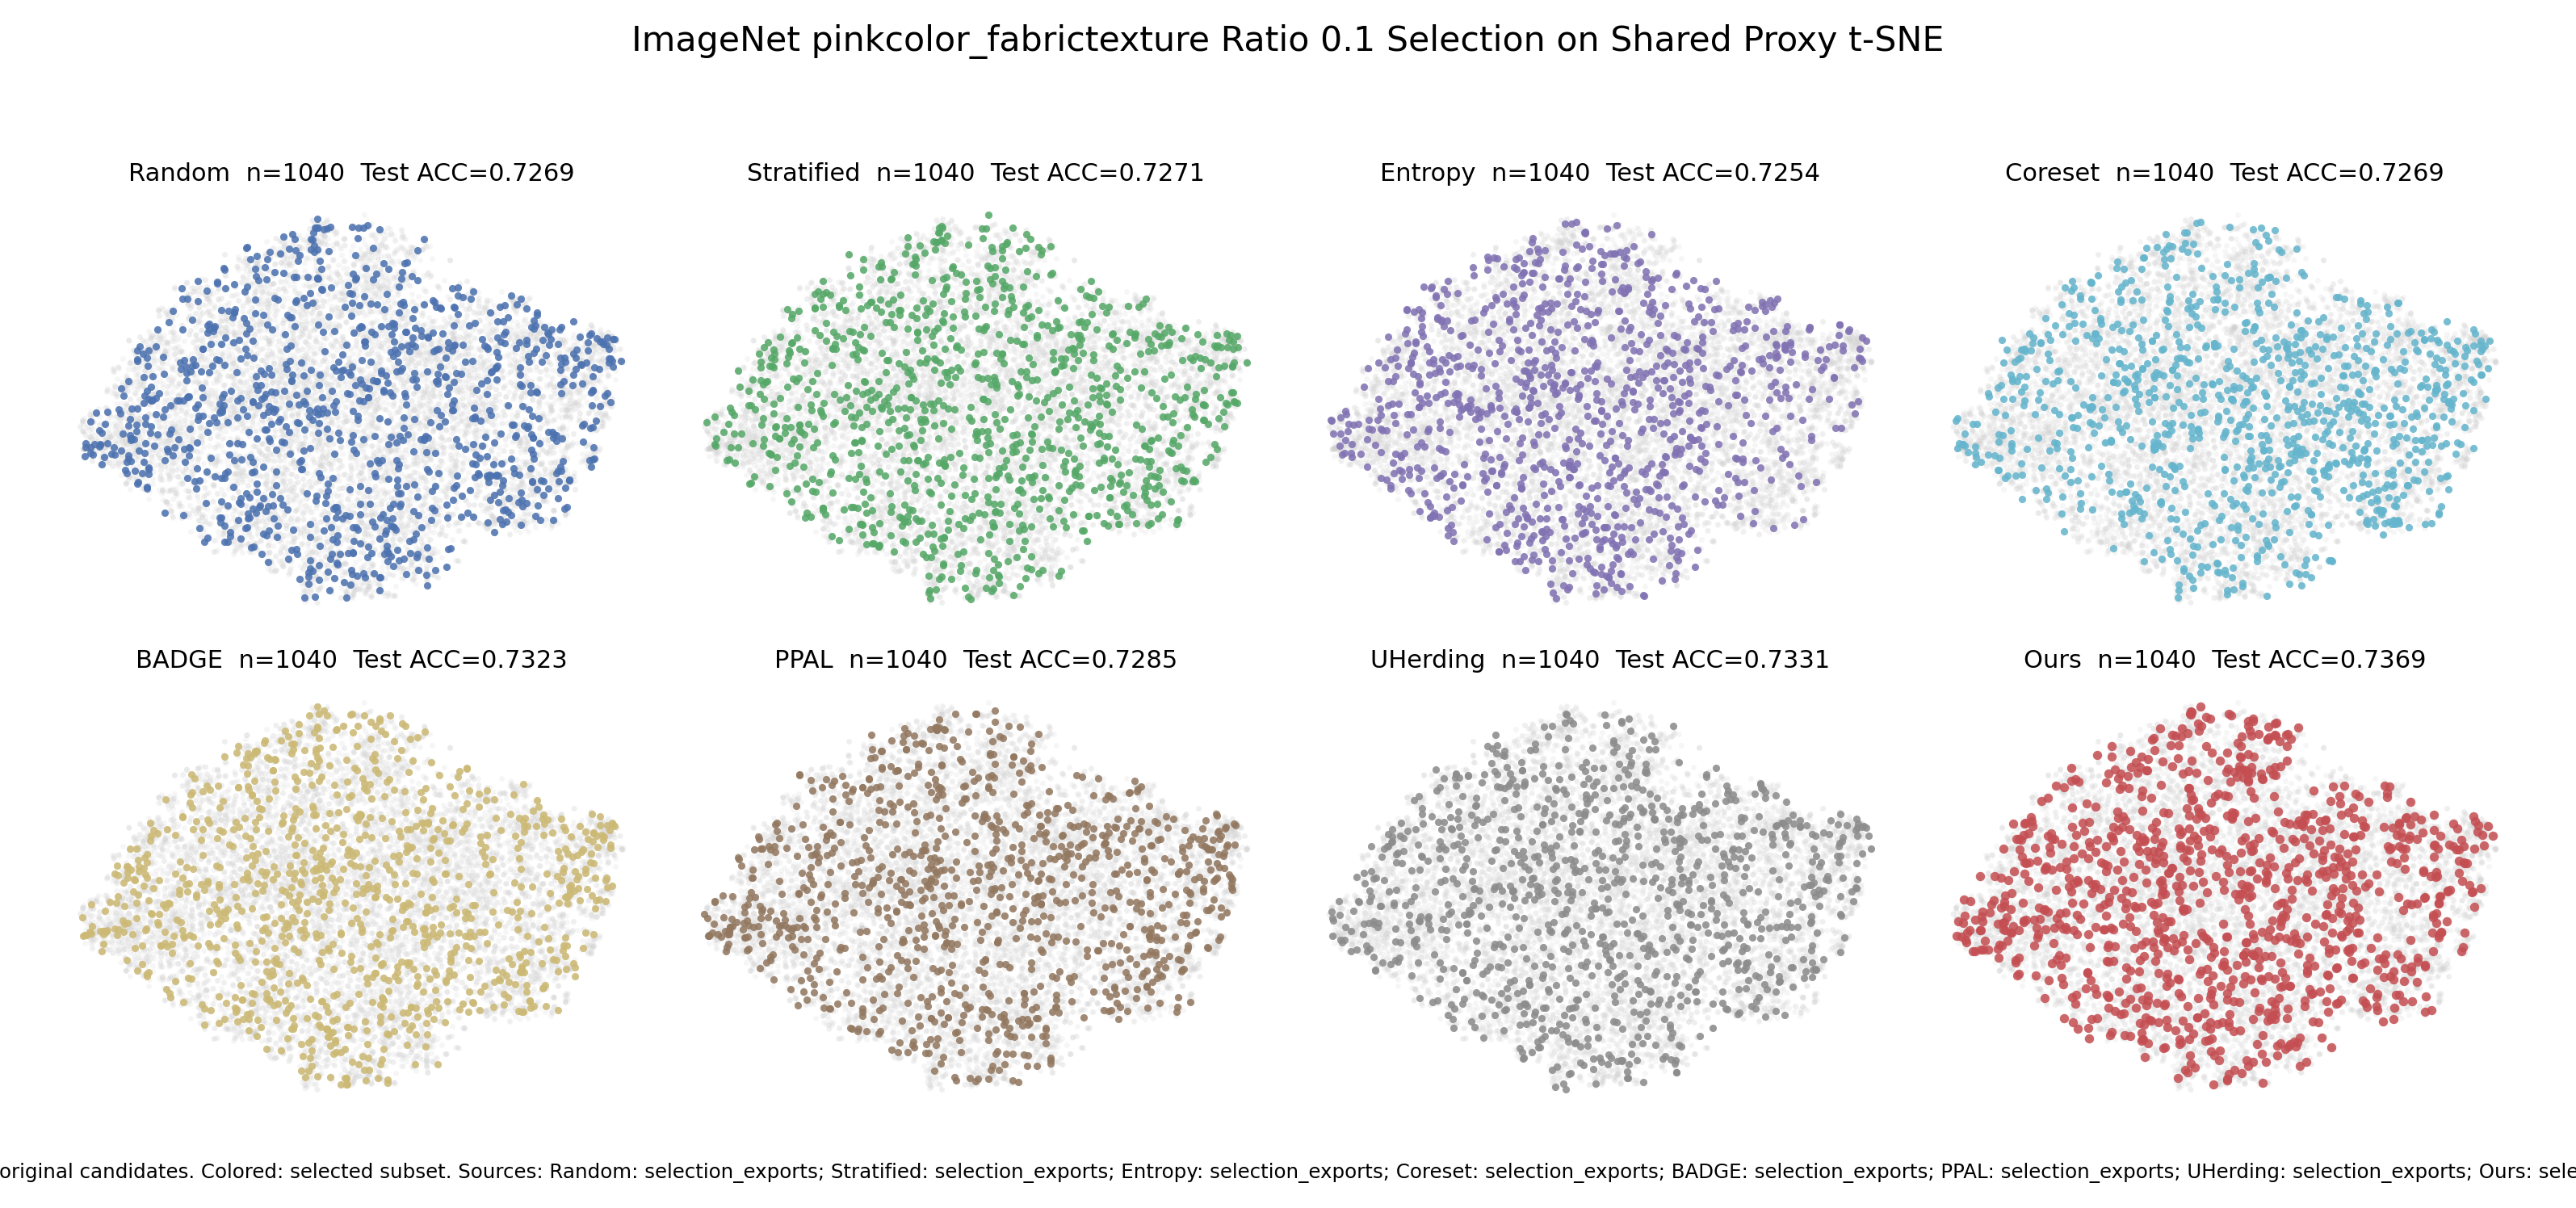
\includegraphics[width=\linewidth]{figures/ratio0p1_selection_tsne/imagenet_controlnet_ratio0p1_selection_tsne.png}
% \caption{ImageNet ratio-$0.10$ selected subsets visualized on a shared source-image t-SNE embedding. Gray points show source candidates; colored points show the subset selected by each method.}
% \label{fig:tsne-r01-imagenet}
% \end{figure}

% \begin{figure}[p]
% \centering
% 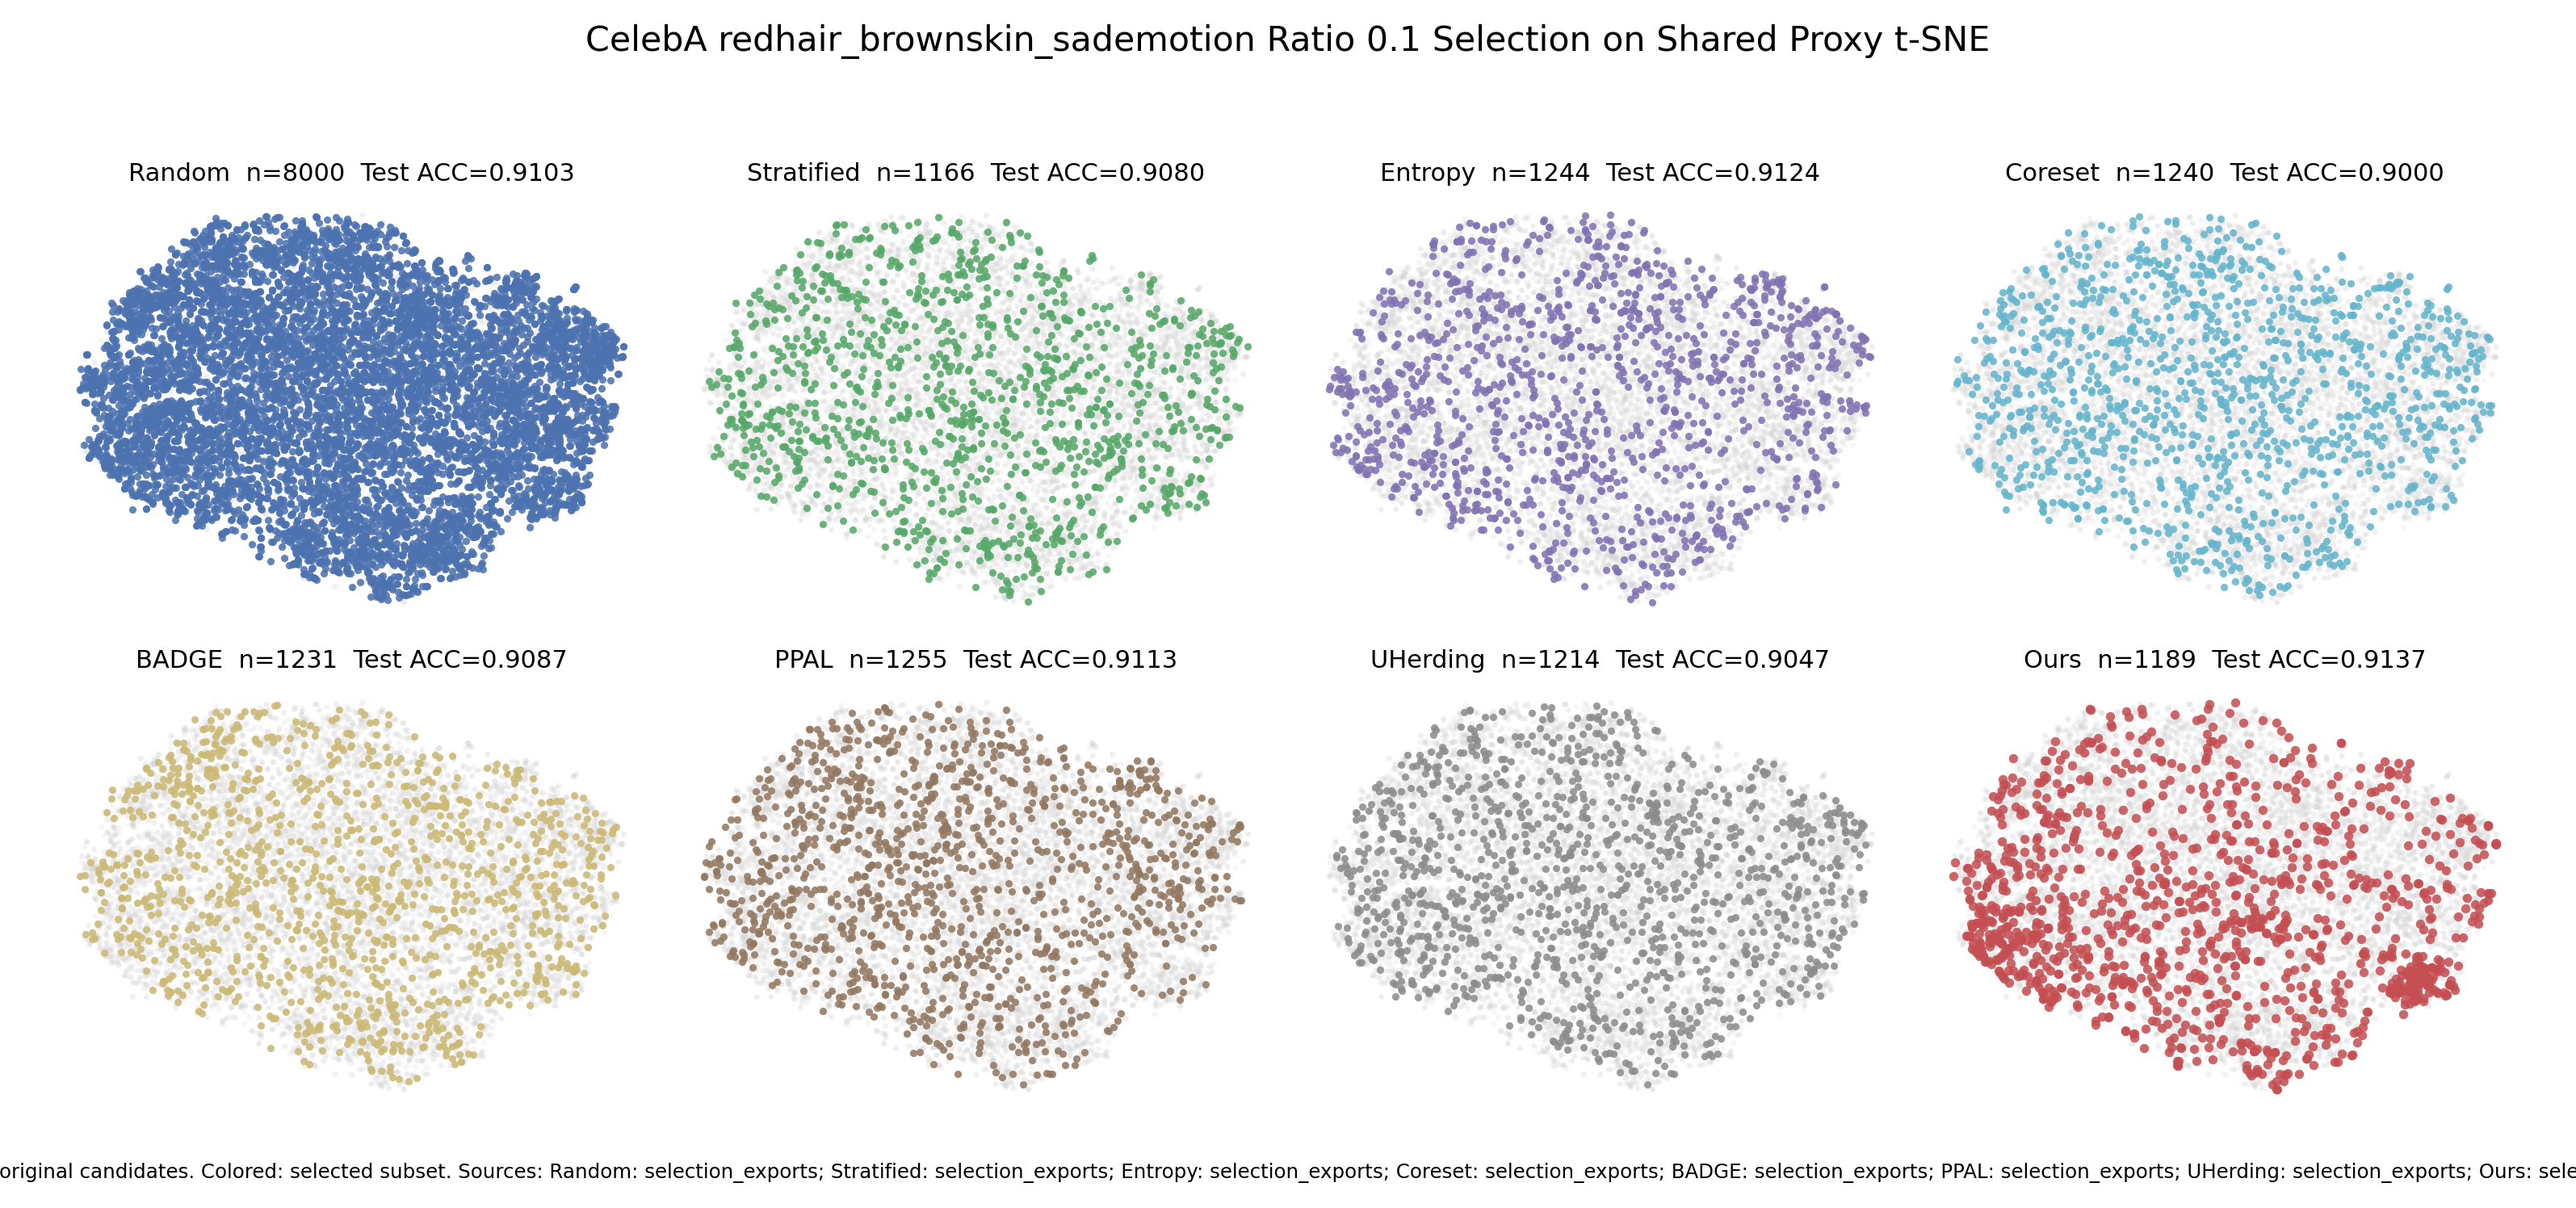
\includegraphics[width=\linewidth]{figures/ratio0p1_selection_tsne/celeba_redhair_brownskin_sademotion_ratio0p1_selection_tsne.png}
% \caption{CelebA ratio-$0.10$ selected subsets visualized on a shared source-image t-SNE embedding.}
% \label{fig:tsne-r01-celeba}
% \end{figure}

\begin{figure}[p]
\centering
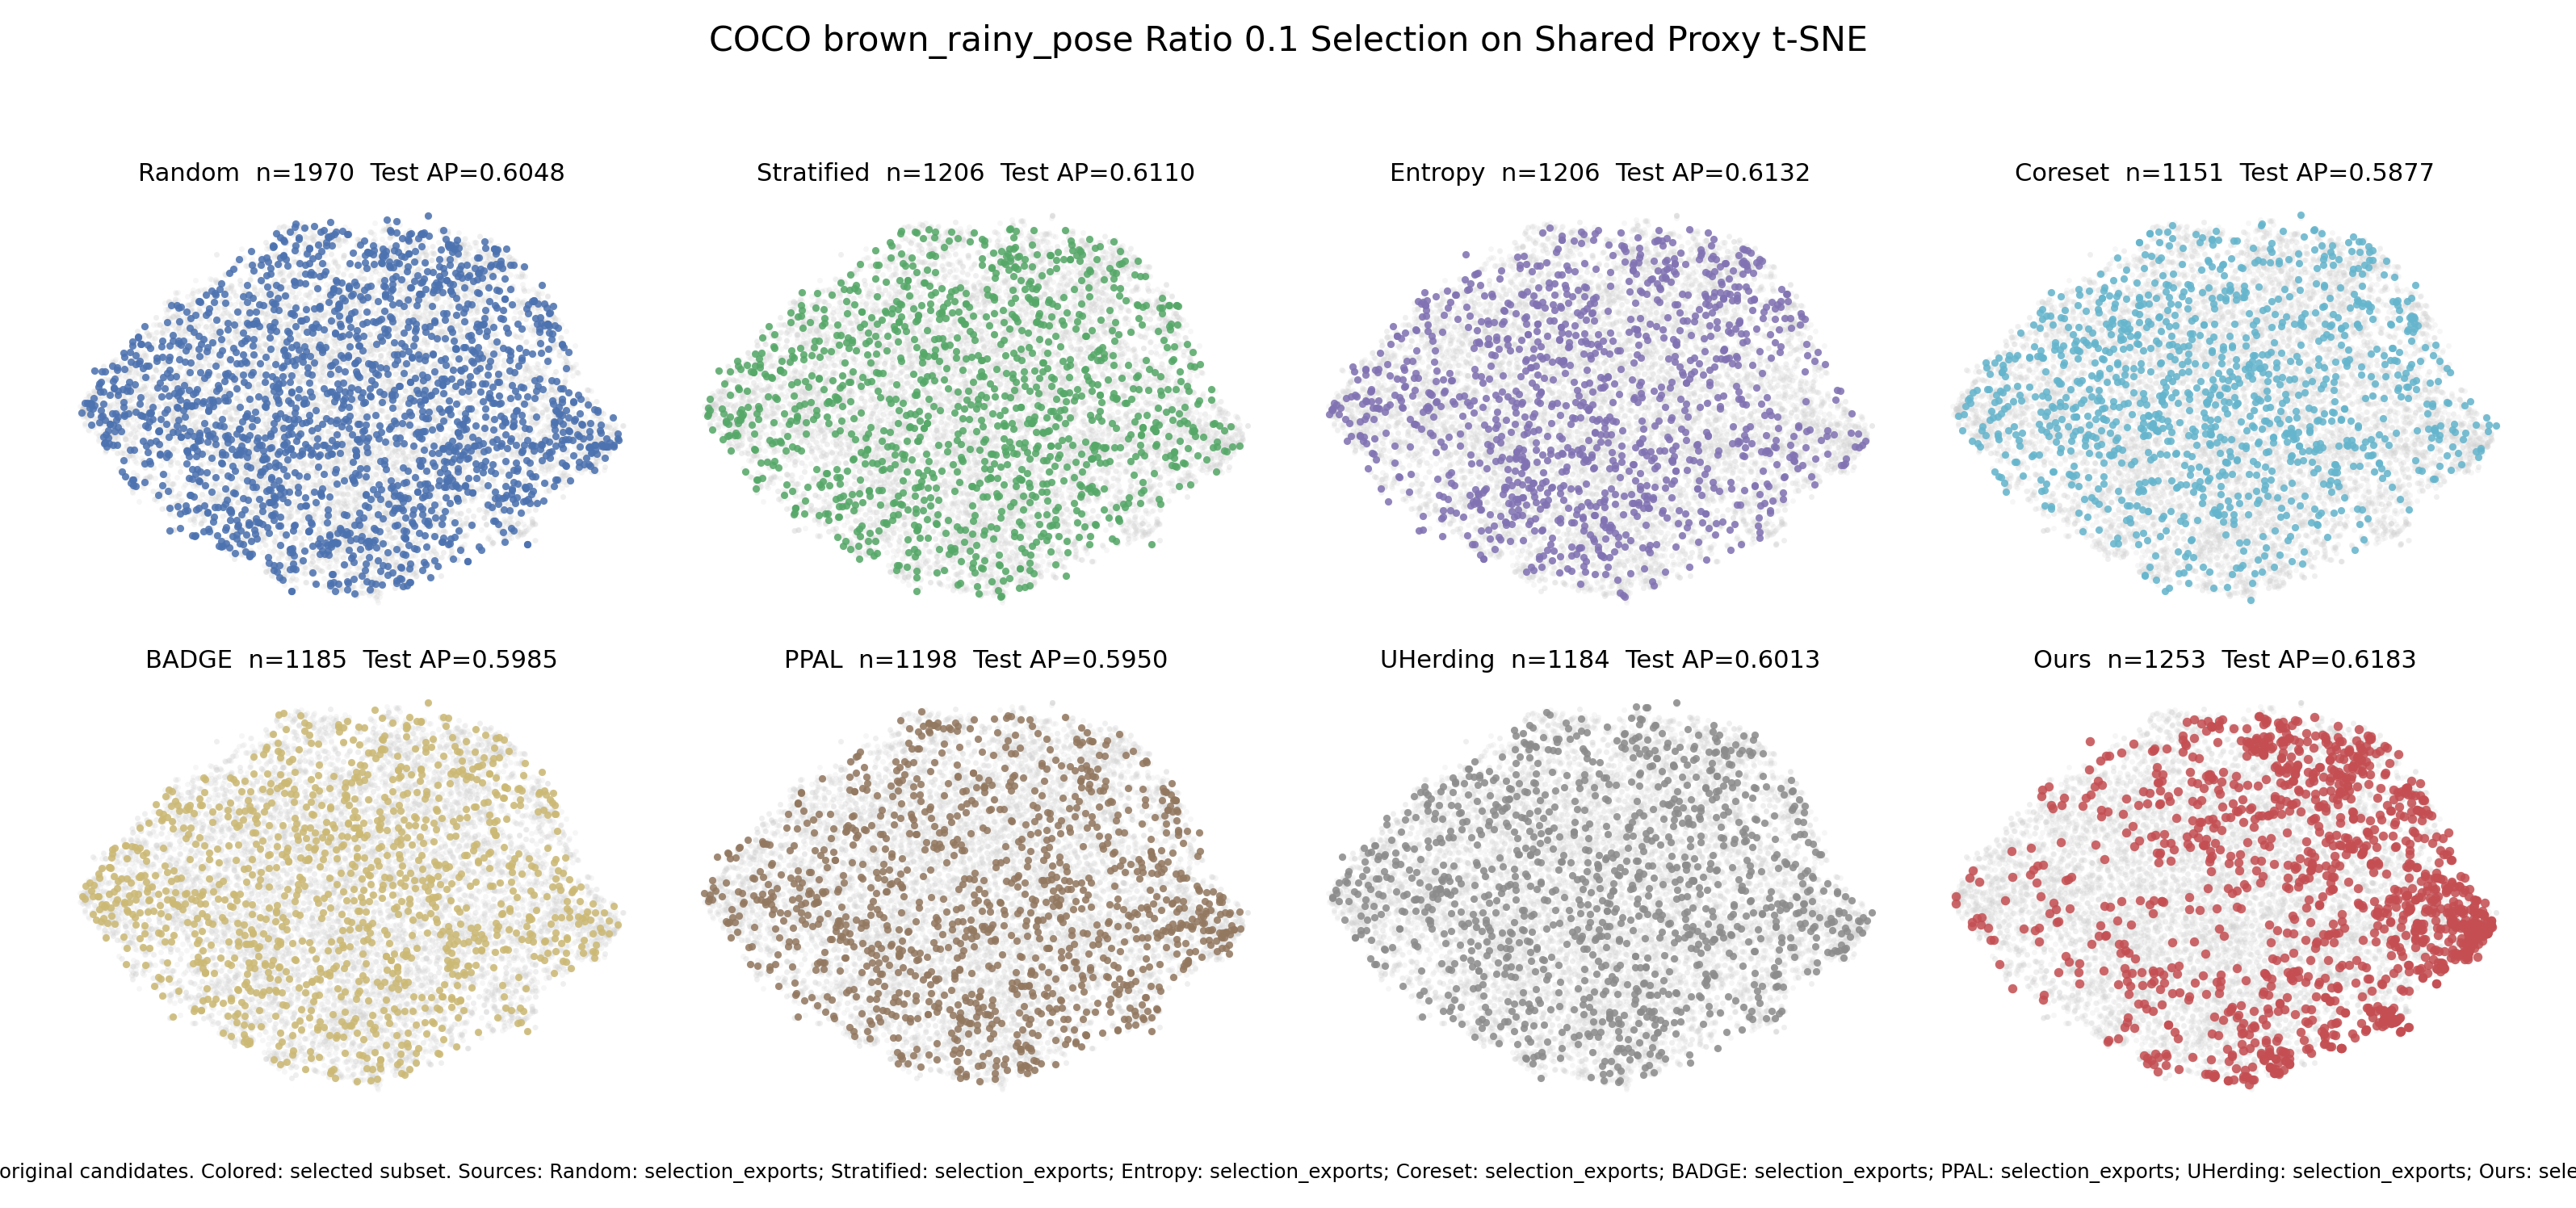
\includegraphics[width=\linewidth]{figures/ratio0p1_selection_tsne/coco_brown_rainy_ratio0p1_selection_tsne.png}
\caption{COCO pose-estimation ratio-$0.10$ selected subsets visualized on a shared source-image t-SNE embedding.}
\label{fig:tsne-r01-coco}
\end{figure}

\begin{figure}[p]
\centering
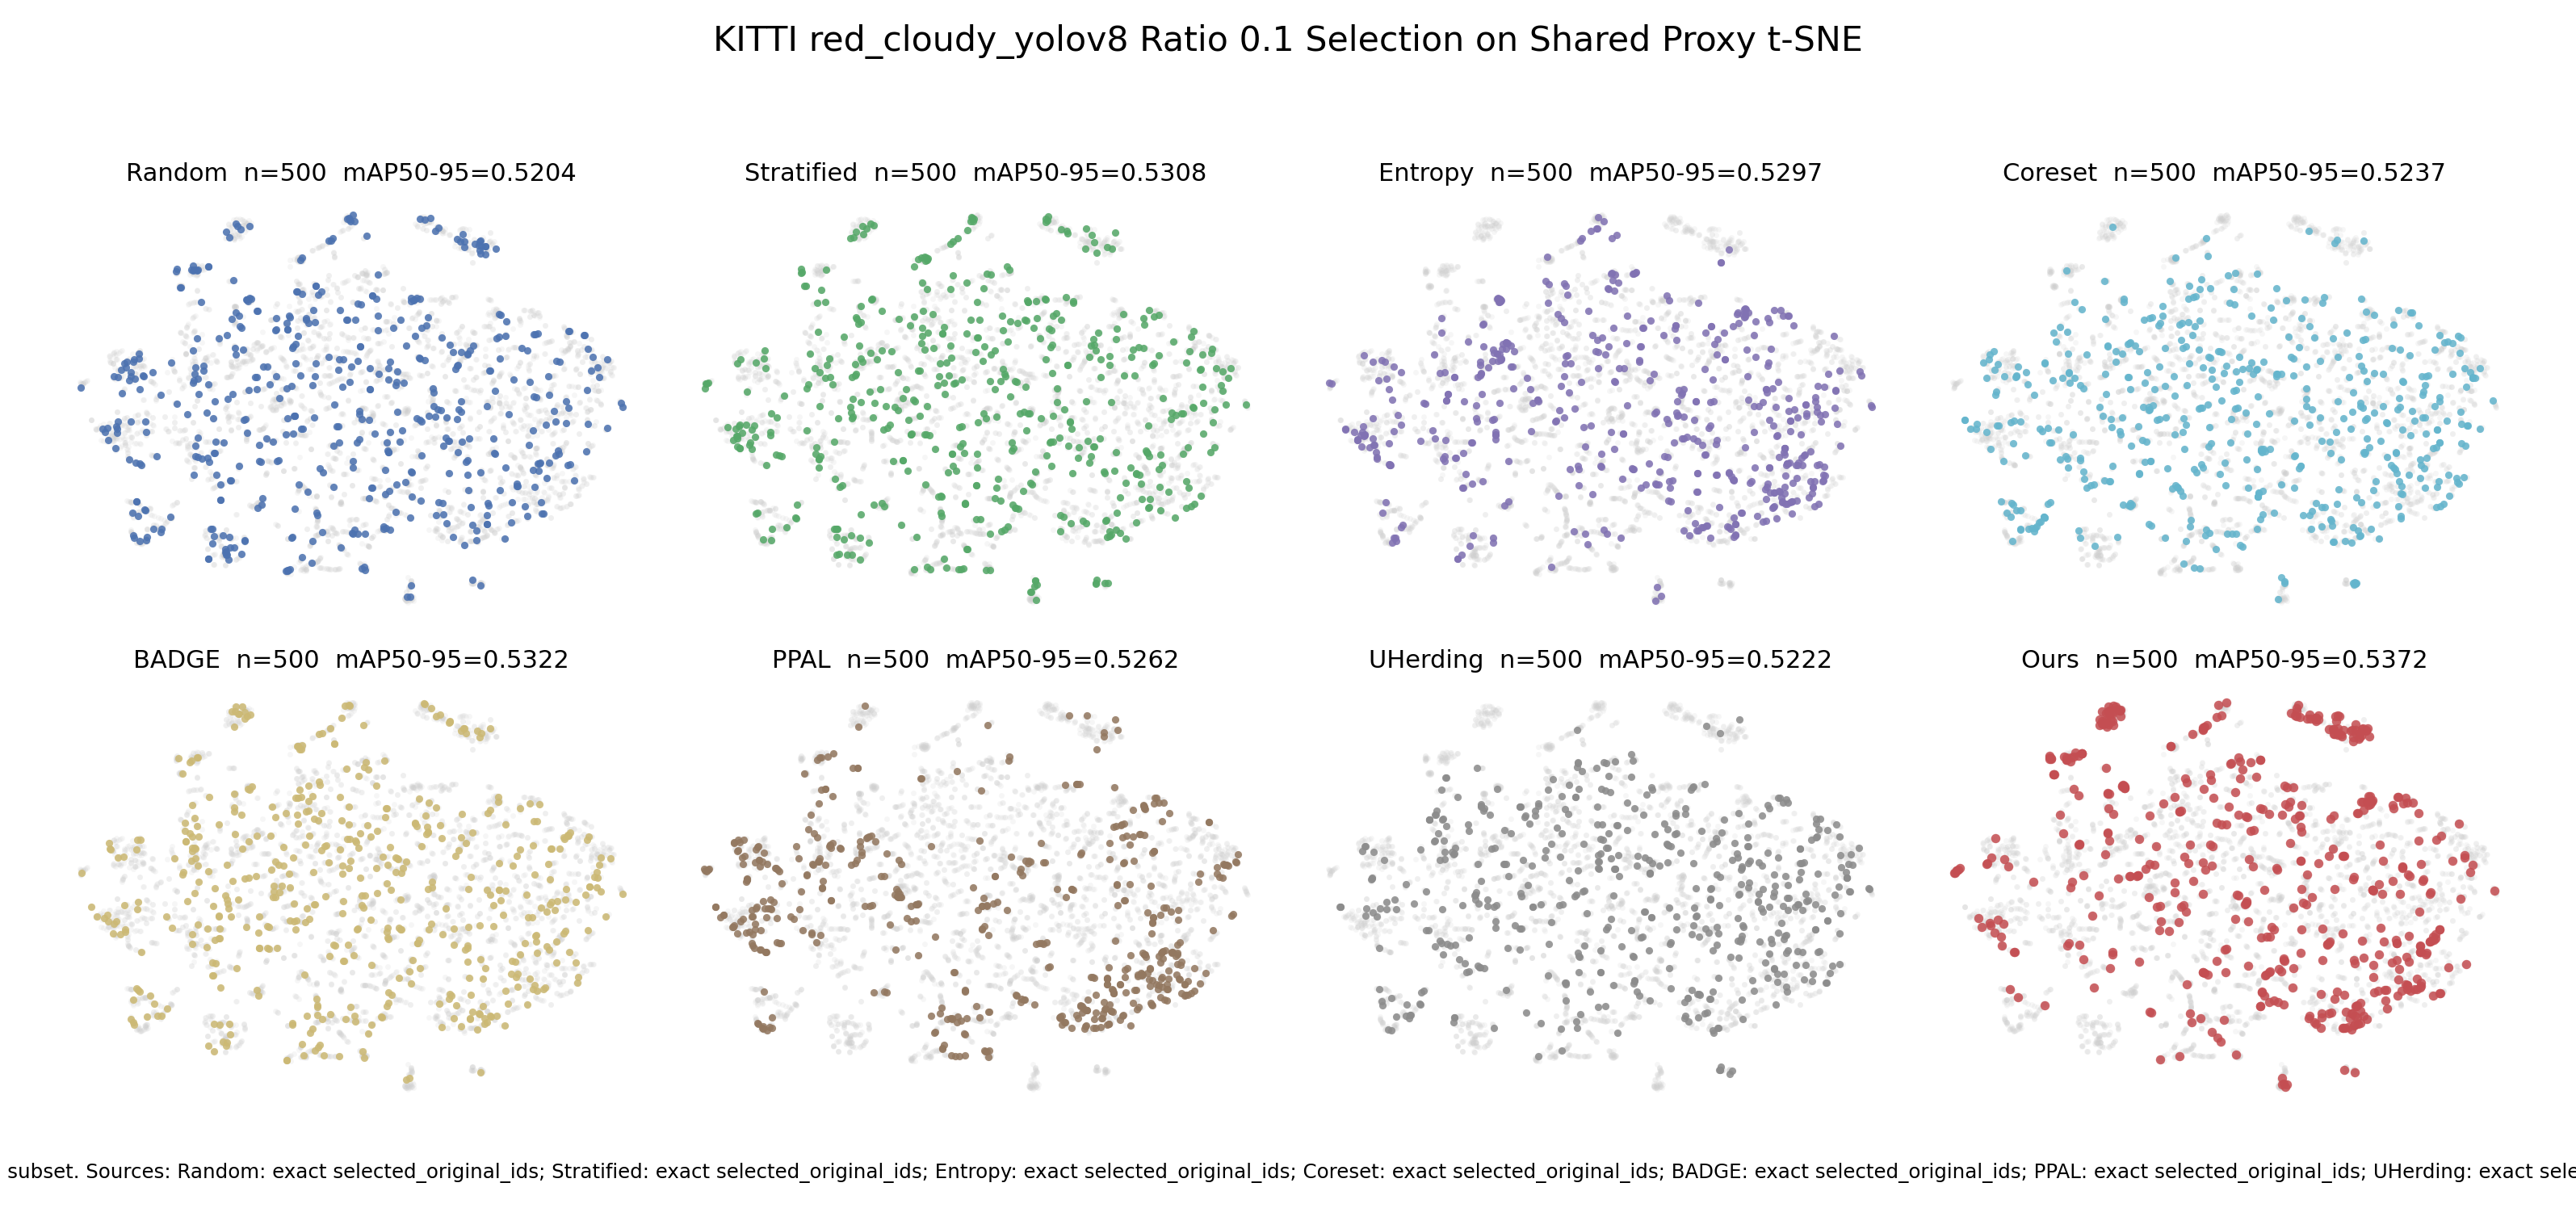
\includegraphics[width=\linewidth]{figures/ratio0p1_selection_tsne/kitti_red_cloudy_ratio0p1_selection_tsne.png}
\caption{KITTI object-detection ratio-$0.10$ selected subsets visualized on a shared source-image t-SNE embedding.}
\label{fig:tsne-r01-kitti}
\end{figure}

% \begin{figure}[p]
% \centering
% 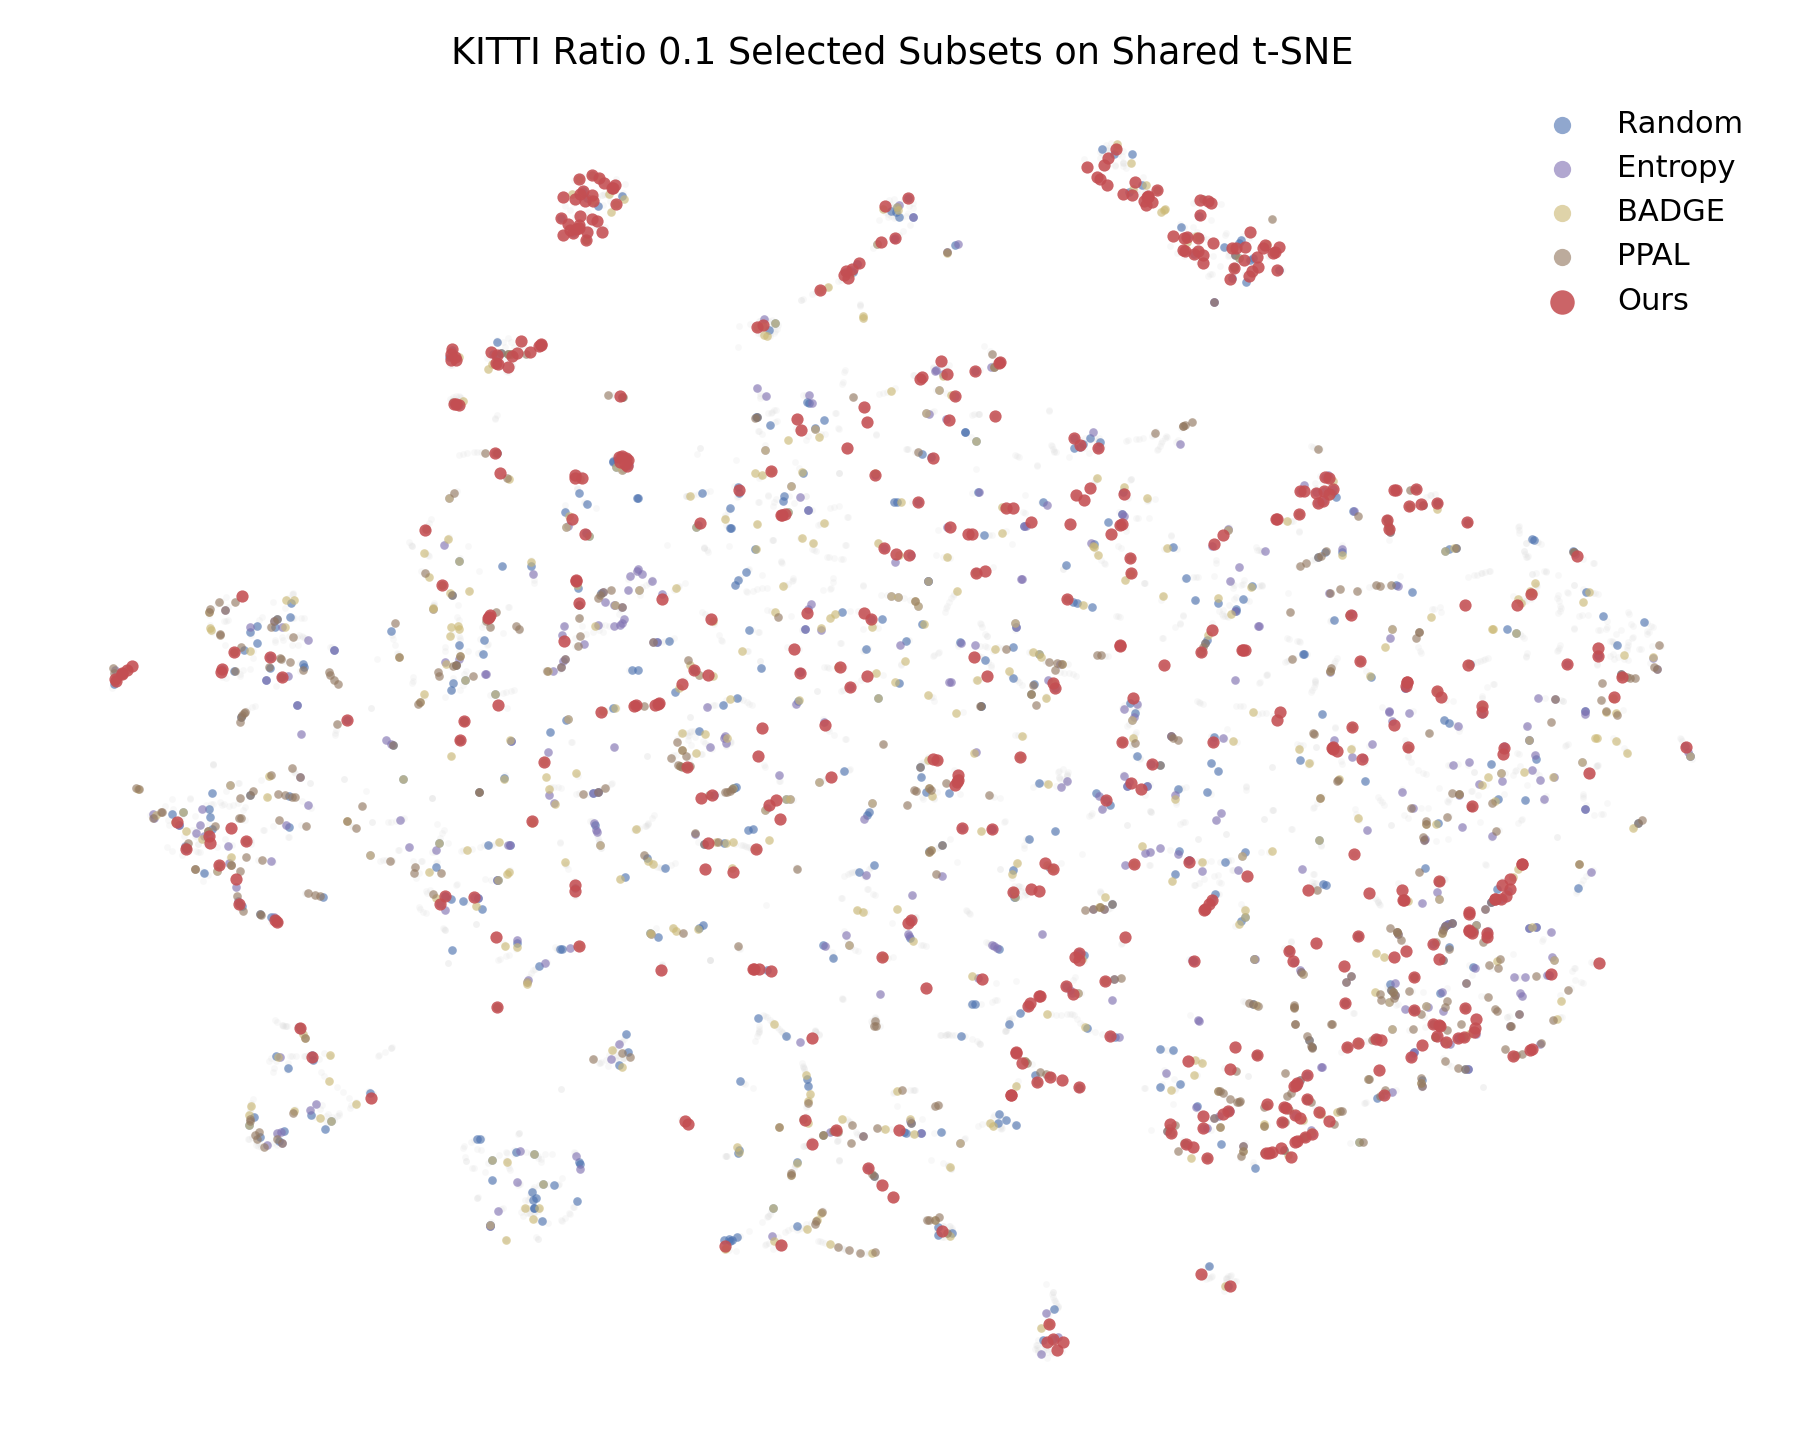
\includegraphics[width=0.86\linewidth]{figures/ratio0p1_selection_tsne/kitti_red_cloudy_ratio0p1_selection_tsne_overlay.png}
% \caption{KITTI object-detection ratio-$0.10$ overlay view for selected active-learning baselines and \model.}
% \label{fig:tsne-overlay-r01-kitti}
% \end{figure}

% \begin{figure}[p]
% \centering
% 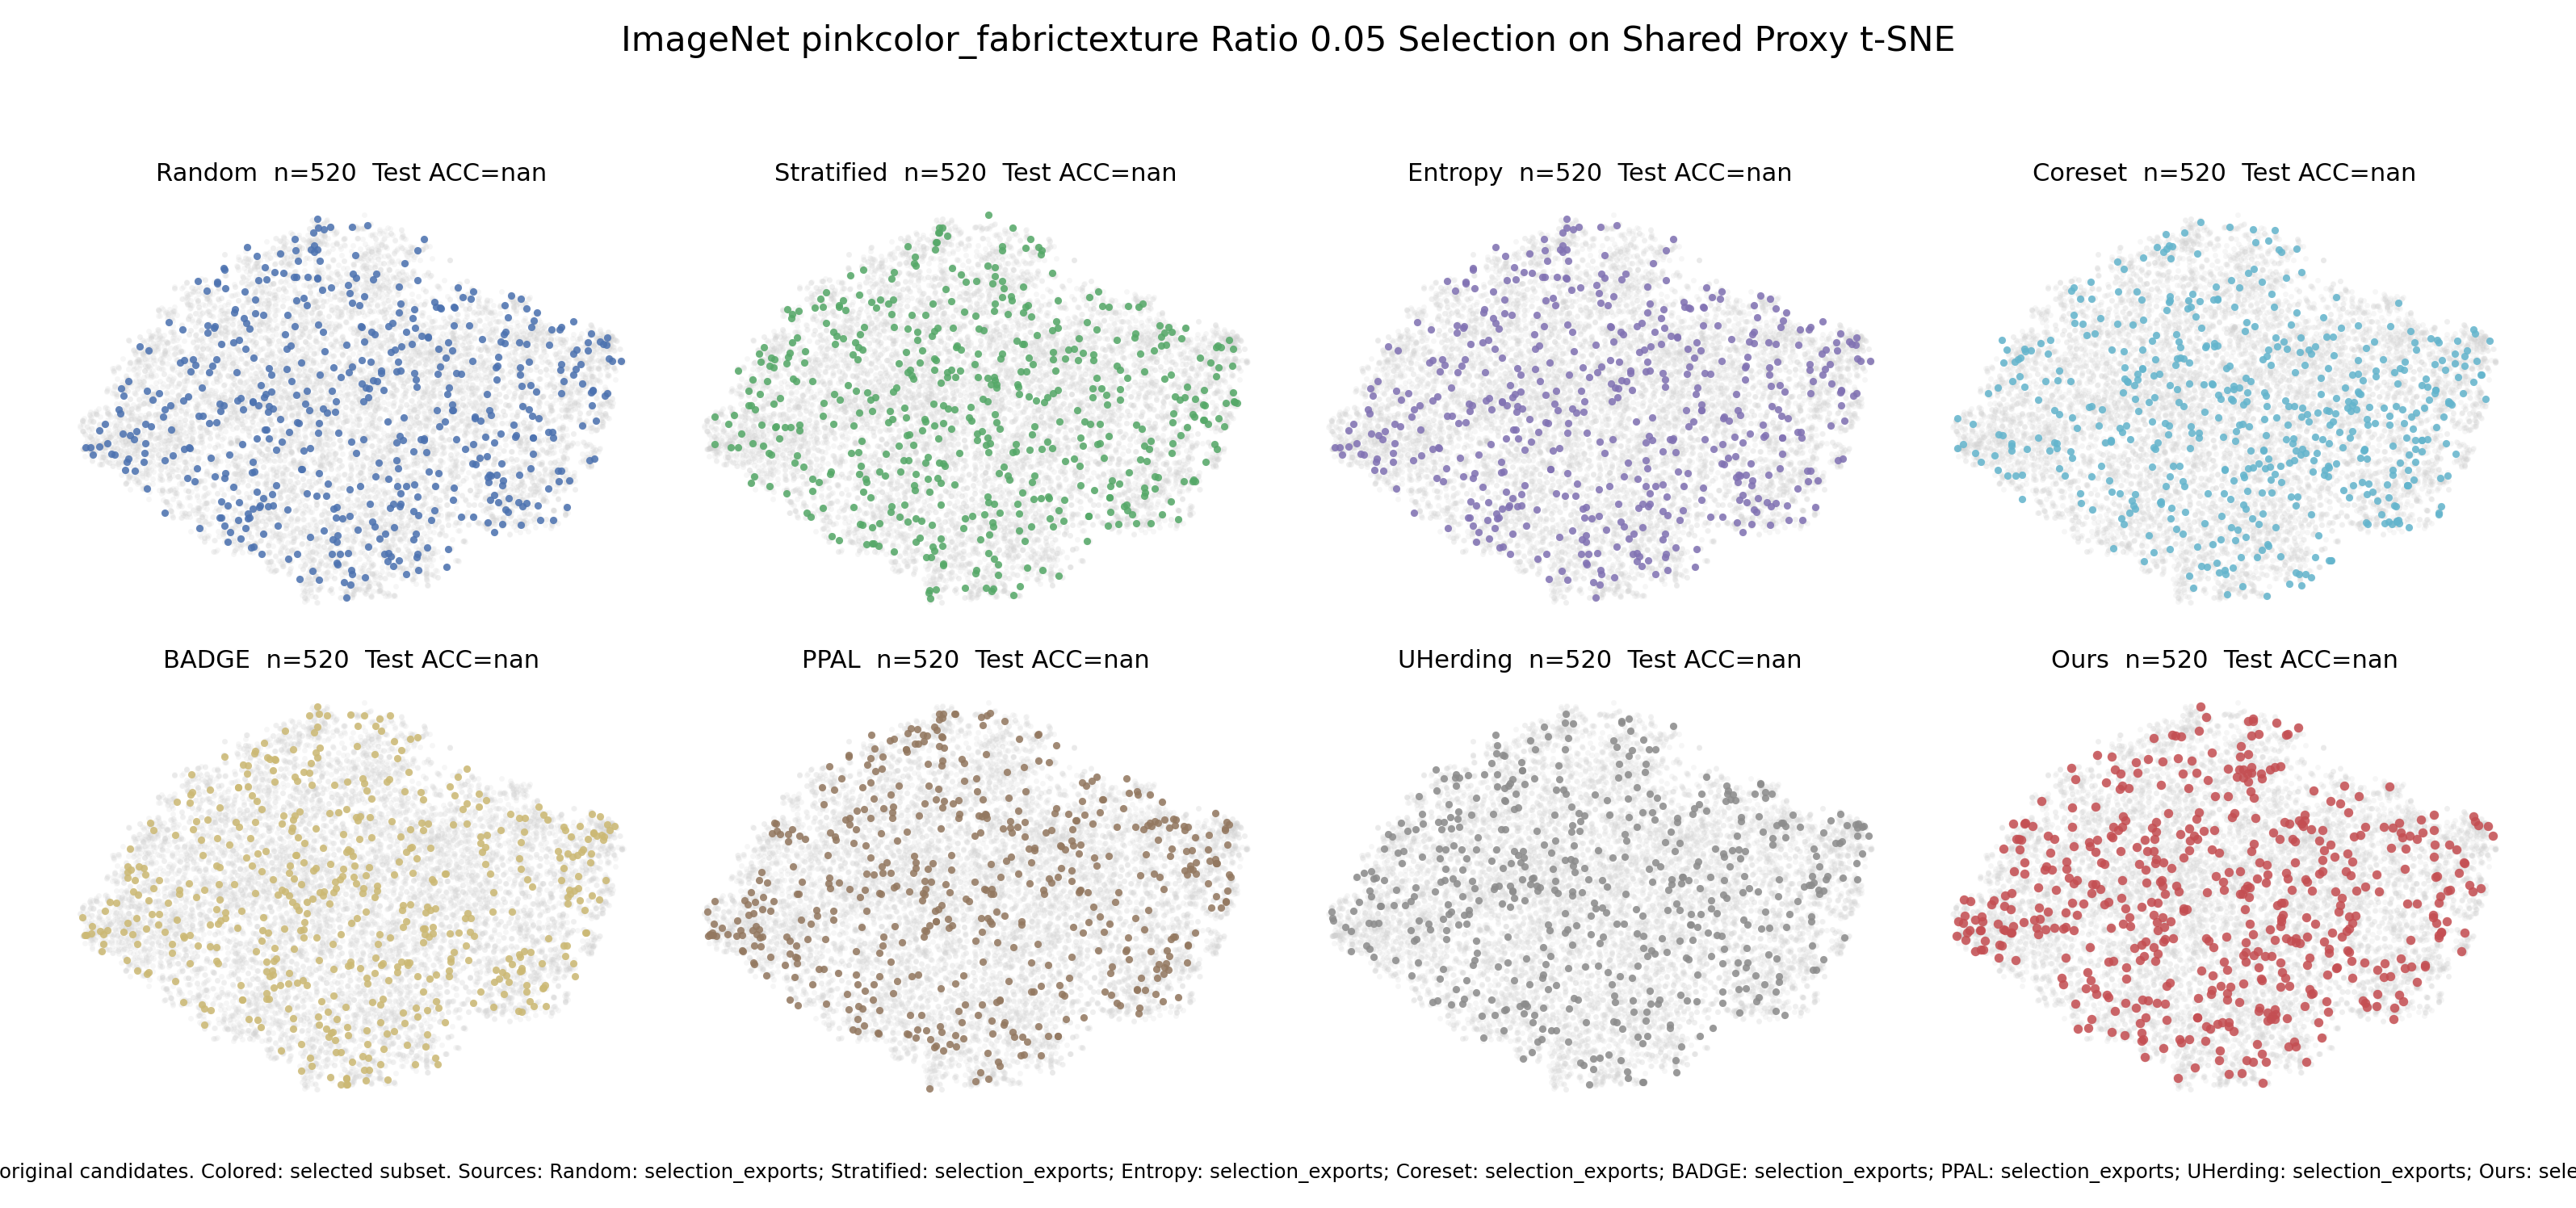
\includegraphics[width=\linewidth]{figures/ratio0p05_selection_tsne/imagenet_controlnet_ratio0p05_selection_tsne.png}
% \caption{ImageNet ratio-$0.05$ selected subsets visualized on a shared source-image t-SNE embedding.}
% \label{fig:tsne-r005-imagenet}
% \end{figure}

\begin{figure}[p]
\centering
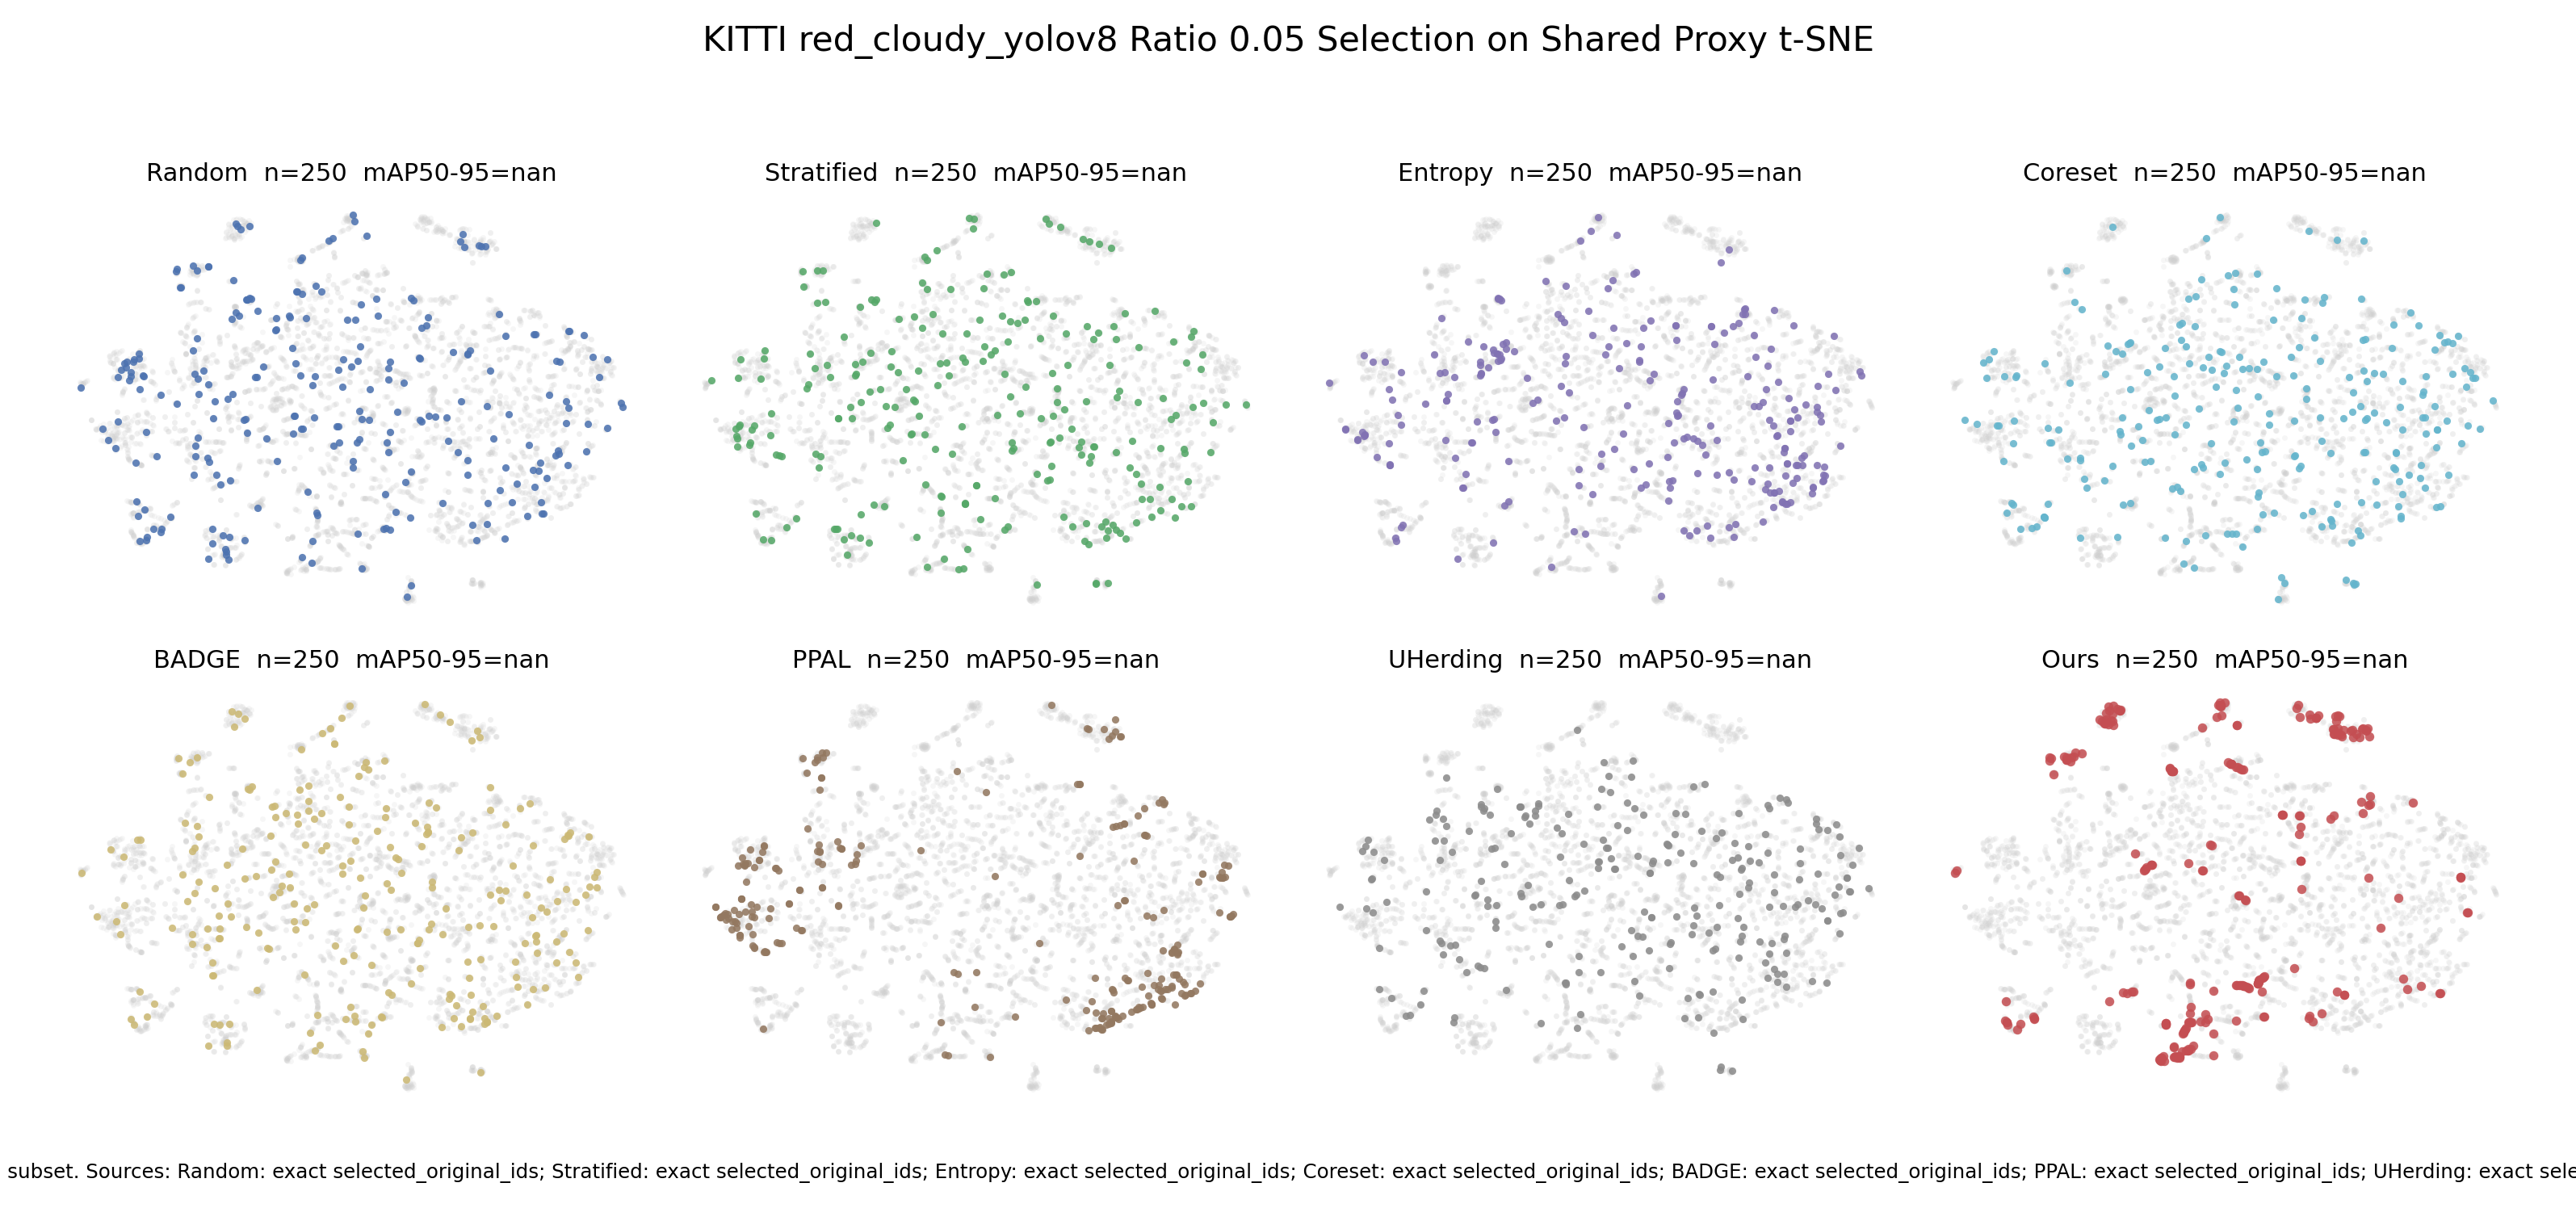
\includegraphics[width=\linewidth]{figures/ratio0p05_selection_tsne/kitti_red_cloudy_ratio0p05_selection_tsne.png}
\caption{KITTI object-detection ratio-$0.05$ selected subsets visualized on a shared source-image t-SNE embedding.}
\label{fig:tsne-r005-kitti}
\end{figure}

\begin{figure}[p]
\centering
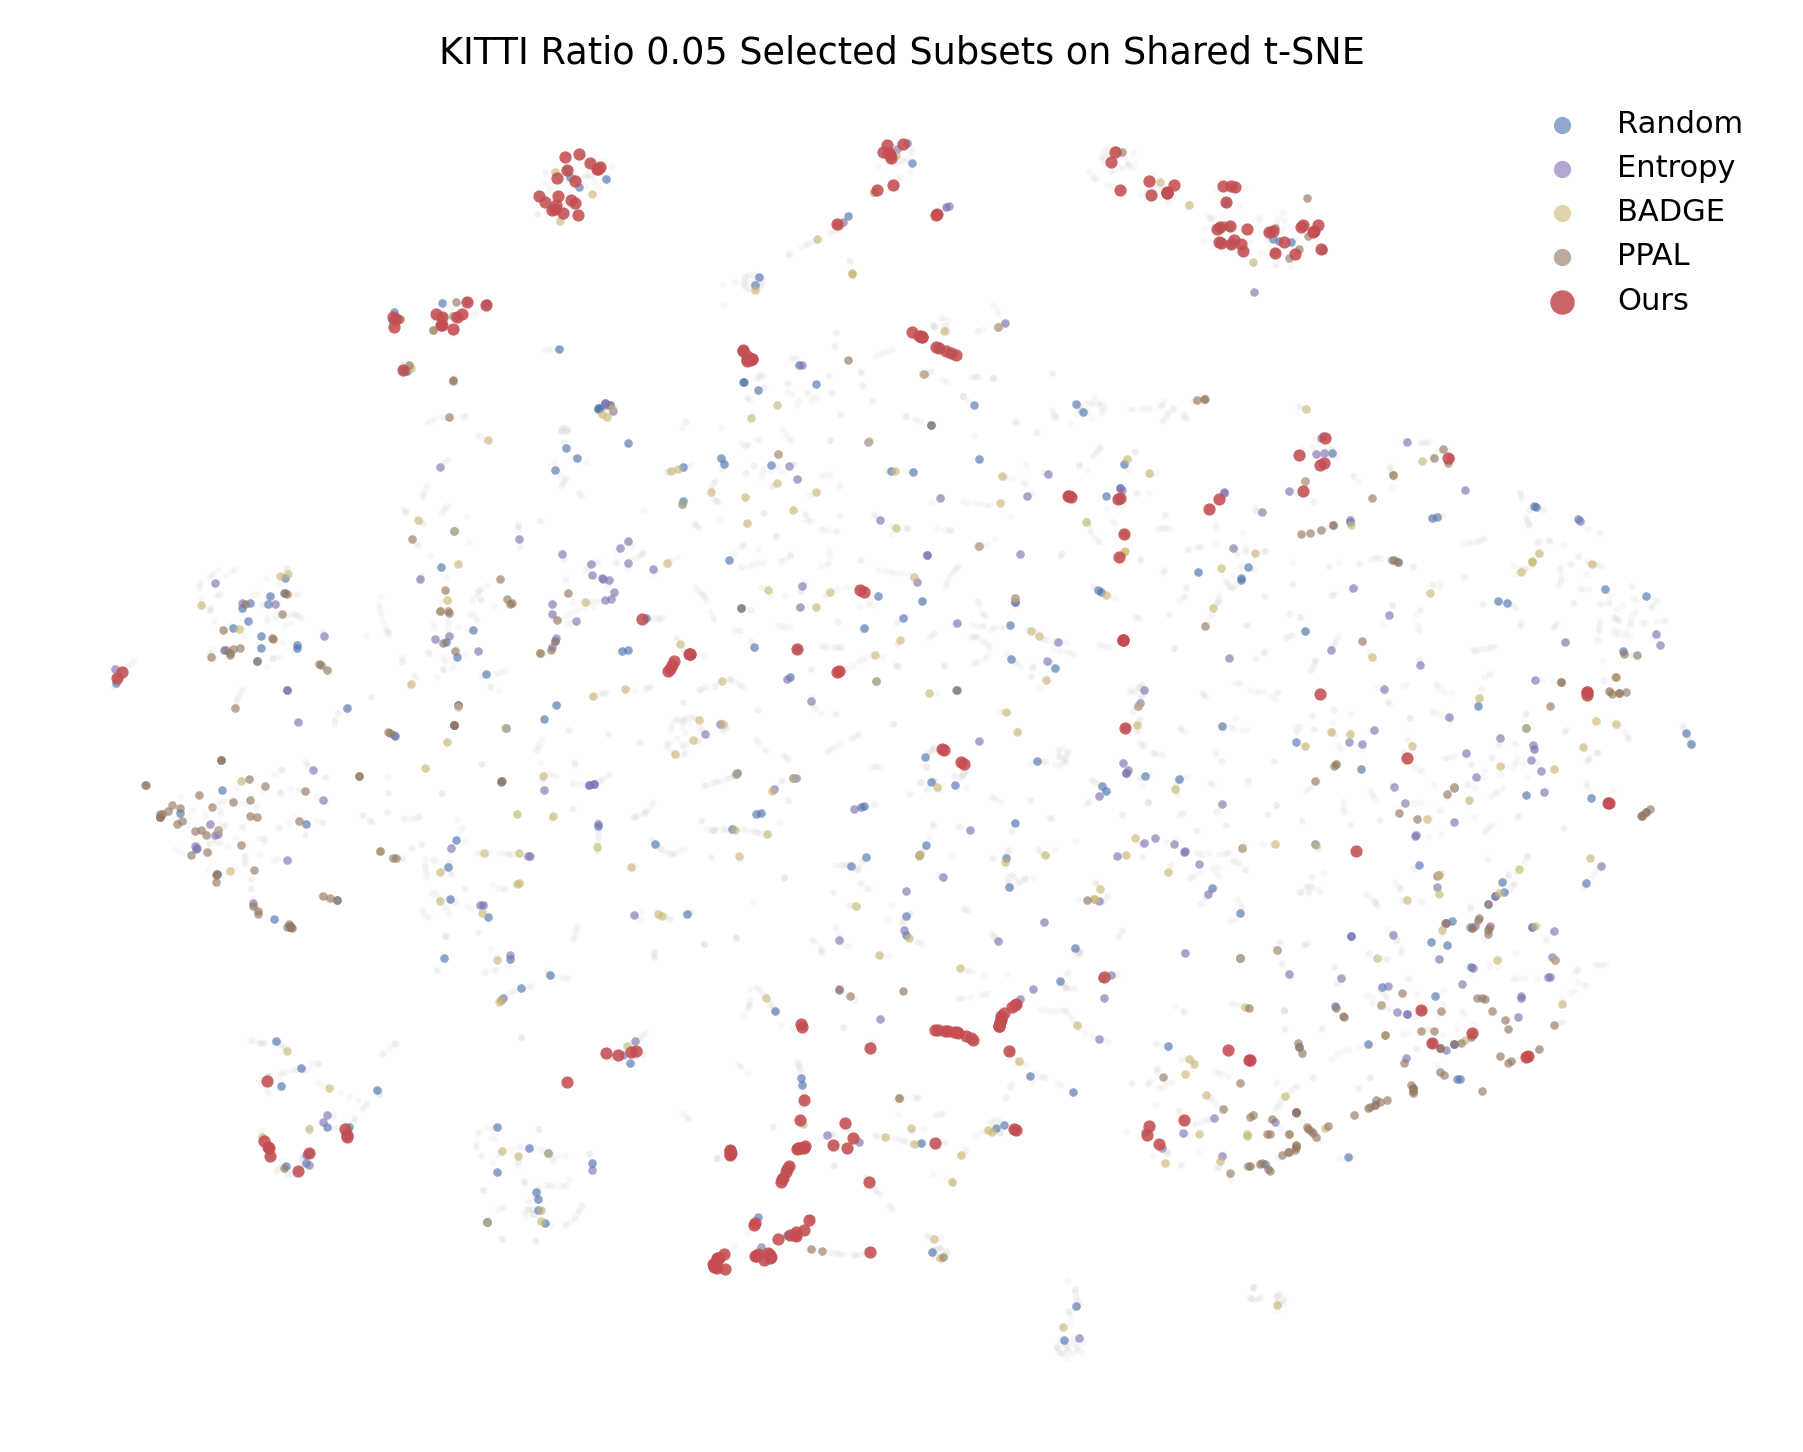
\includegraphics[width=0.86\linewidth]{figures/ratio0p05_selection_tsne/kitti_red_cloudy_ratio0p05_selection_tsne_overlay.png}
\caption{KITTI object-detection ratio-$0.05$ overlay view for selected active-learning baselines and \model.}
\label{fig:tsne-overlay-r005-kitti}
\end{figure}

\clearpage

